\documentclass{beamer}
\usepackage{fontspec}
\usepackage{thesis}
\usetheme{metropolis}

\newfontfamily\zafont{MingLiU}
\newfontfamily\zbfont{MingLiU_HKSCS-ExtB}

\title{Our Names in the Computing Age}
\date{\today}
\author{Gabe DeFreitas}

\begin{document}

\maketitle

\begin{frame}{A Survey of Names}
\textbf{United States}: Personal; Middle; Family \\
\textbf{Latin America/Spanish}: Personal; Middle; Patronym; Matronym \\
\textbf{South India}: Personal; Family; Village \parencite{finch08} \\
\textbf{Japan}: Family; Given \\
\textbf{Hungary}: Family; Given \\
\textbf{China}: Family; First character; Second character \parencite{louie06}\\
\textbf{Iceland}: Given; Father's given \textit{-son/dottir}; \\
\textbf{Pakistan}: Given; Father's given \\
\textbf{Nuer (Sudan)}: Maternal given; Paternal given; Clan; Ox; Nickname(s)
\parencite{wardhaugh92} \\
\end{frame}

\begin{frame}{Functions of a Name}
\begin{itemize}
\item \textbf{Reference function}: A linguistic token that identifies an
individual. ("Who is that? That is John.")
\item Names help us select people from our "social database" in order to view
the full "entry".
\item \textbf{Social Function}: But names do more than refer to a human entity.
\end{itemize}
\end{frame}

\begin{frame}{A Very Infamous Name}
\begin{aquote}{J.K. Rowling}
"Sir?" said Harry. "I've been thinking…sir—even if the Stone’s gone, Vol-, I
mean, YouKnow-Who—" \\ "Call him Voldemort, Harry. Always use the proper name for
things. Fear of a name increases fear of the thing itself."
\end{aquote}
\end{frame}

\begin{frame}{Connecting and Individualizing Functions}
\begin{itemize}
\item \textbf{Connecting Functions}: Personal names place you in a social,
linguistic, ancestral context (We-Identity)
\item \textbf{Individualizing Functions}: Parents choose a name to evoke some
desired quality in a child; a name is what makes You You! (I-Identity)
\item The forename-surname paradigm captures this contrast, although this may be
modified, for example when a child's given name is the name of an ancestor.
\end{itemize}
\fullcite{finch08}
\end{frame}

\begin{frame}{A Need for Standardized Naming Practices}
\begin{itemize}
\item Modern governments require organized data about its populations to carry
out large-scale plans.
\item Need to quickly and accurately identify individuals; reference function of
names has become more important.
\item Surnames narrow the chances of misidentification and provide information
about an individual's family and ancestry.
\end{itemize}
\fullcite{scott02}
\end{frame}

\begin{frame}{Scott et. al.}
\begin{aquote}{\textcite{scott02}}
The rise of the permanent patronym is inextricably associated with those aspects
of state-making in which it was desirable to distinguish individual (male)
subjects: tax collection (including tithes), conscription, land revenue, court
judgements, witness records, and police work.
\end{aquote}
\end{frame}

\begin{frame}{An Example}
\begin{center}
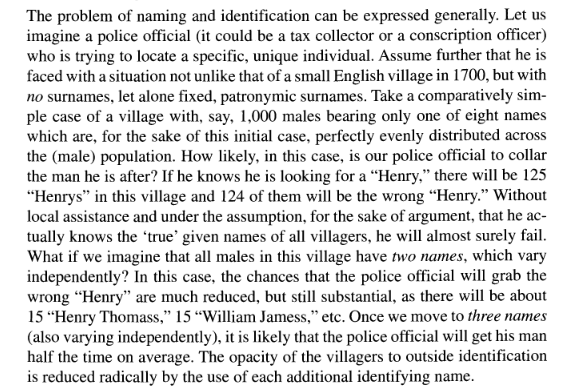
\includegraphics[scale=0.4]{subtex/scott9.png}
\end{center}
\end{frame}

\begin{frame}{Computers}
\begin{itemize}
\item Digital society is accelerating the degradation of names' social
function.
\item Large-scale digital communication (ie. globalisation) is levelling the
\end{itemize}
\end{frame}

\begin{frame}{Thus Spake Lord Zuckerberg}
\begin{aquote}{Facebook}
Facebook is a community where everyone uses the name they go by in everyday
life. This makes it so that you always know who you're connecting with. Your
name can't include:
\begin{itemize}
\item Symbols, numbers, unusual capitalization, repeating characters or punctuation.
\item Characters from multiple languages.
\item Titles of any kind (example: professional, religious).
\item Words or phrases in place of a name.
\end{itemize}
\end{aquote}\textcite{what-names-fb}
\end{frame}

\begin{frame}{California}
\begin{itemize}
\item 29\% of California's population speaks Spanish in the home.
\textcite{acs-lang-states}
\item However, English was declared the official language by a 1986 ballot
referendum; the legislature has the power to enforce this provision by law.
\item Accordingly, the Office of Vital Records prohibits the use of non-English
characters in birth certificates; likewise for drivers licenses.
\parencite{larson11}
\item A 2017 bill to allow diacritical marks passed both houses of the
legislature but was vetoed by Governor Brown because computer upgrades were
expected to cost millions of dollars.
\end{itemize}
\end{frame}

\begin{frame}{China}
\begin{itemize}
\item Mǎ Chěng's ({\zafont 马}{\zbfont 𩧢}) given name is not one of the 32,252 characters recognised
by government computers in China.
\item In 2009, \textit{New York Times} reported that Chinese government was
introducing new ID cards;
\item "Miss Ma and at least some of the 60 million other Chinese with obscure
characters in their names cannot get new cards — unless they change their names
to something more common." \parencite{lafraniere09}
\item At the time of the article, Mǎ solved the problem by obtaining a
temporary ID card every three months.
\end{itemize}
\end{frame}

\begin{frame}{Hawaii}
\begin{itemize}
\item Hawaiian woman Janice Lokelani Keihanaikukauakahihuliheekahaunaele won a
battle with the state government in 2013 to have her full name included on her
driver's license.
\item Her lengthy surname is her deceased husband's complete name.
\item Hawaiian is one of two official languages in the State of Hawaii, the
other being English.
\end{itemize}
\begin{aquote}{Janice "Lokelani" Keihanaikukauakahihuliheekahaunaele}
Over the last 22 years I have seen...the culture of Hawaii being trampled upon
and this policeman treated my name as if it was mumbo-jumbo.
\end{aquote}
\end{frame}

\begin{frame}{Lithuania}

i

\end{frame}

\begin{frame}{Solutions and Strategies}

\begin{itemize}
\item Unicode
\item Passports
\item More
\end{itemize}

\end{frame}

\begin{frame}[allowframebreaks]{References}

\printbibliography

\end{frame}

\end{document}
